%%%%%%%%%%%%%%%%%%%%%%%%%%%%%%%%%%%%%%%%%%%%%%%%%%%%%%%%%%%%%%%%%%
%%%%%%%%%%%%%%%%%%%%%%%%%%%%%%%%%%%%%%%%%%%%%%%%%%%%%%%%%%%%%%%%%%

\subsection{Introduction}
Pour rappel, notre \acrshort{os} est exécuté sur architecture Intel 32-bits (\acrshort{IA-32})
en mode protégé. Dans cette architecture, quatre niveaux de privilèges existent.
Nous avons déjà fait référence aux niveaux de privilèges (ou \textit{ring})
dans ce document quand les différentes tables de descripteurs ont été décrites
(chapitres \ref{gdt_ldt} sur la \acrshort{gdt} et la \acrshort{ldt} et \ref{idt}
sur l'\acrshort{idt}). Les niveaux de privilèges vont de 0 à 3. Le \textit{ring}
0 (\textit{kernel}) a le plus de privilèges et peut accéder à tout le jeu d'instructions
du processeur alors que le \textit{ring} 3 (\textit{user}) en a le moins et a accès
à un jeu d'instructions restreint \cite{ref42}.

\begin{figure}[!h]
  \centering
  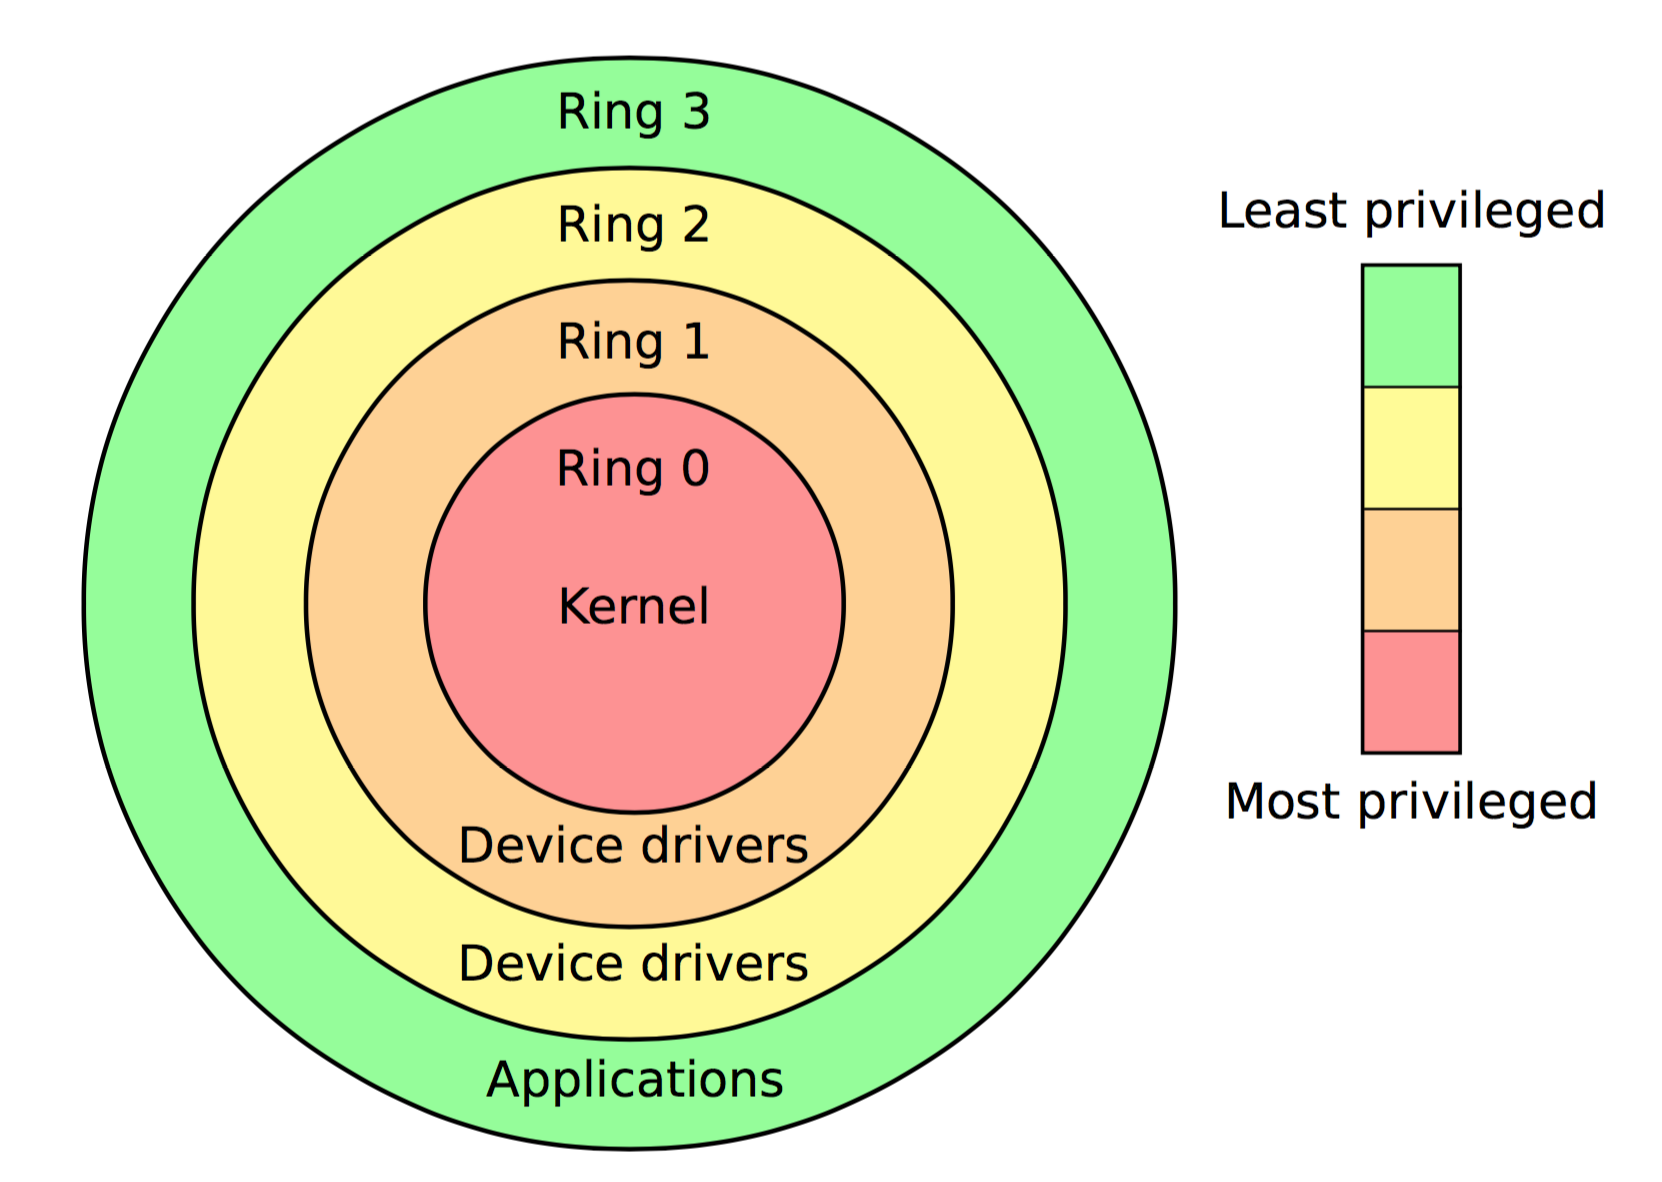
\includegraphics[scale=.4]{images/rings.png}
  \caption{Niveaux de privilèges sur architecture \acrshort{IA-32}}
  \label{gdt}
\end{figure}

Le \textit{ring} 0 est aussi appelé mode privilégié. Ce mode peut accéder aux régions
privilégiées de la mémoire (définies lors de l'initialisation de la \acrshort{gdt}
ou de la pagination). Seulement ce mode peut contrôler le \acrshort{mmu}, accéder
aux périphériques, définir les vecteurs d'interruptions ou encore arrêter le
processeur. L'\acrshort{os} démarre en mode privilégié car le \textit{kernek} doit
pouvoir accéder au matériel sans aucune restriction. Si ce n'était pas le cas toutes
les configurations de la mémoire et des périphériques décrites dans ce document
auraient été impossibles. En revanche, Les applications utilisateur s'exécutent
en mode utilisateur (\textit{ring} 3). Si une application utilisateur démarrait
avec le niveau de privilèges maximal, elle pourrait écrire dans les régions mémoires
du \textit{kernel}, modifier la configuration de la mémoire (\acrshort{gdt} ou 
répertoire de pages) ou encore changer l'\acrshort{idt}. Il est donc impératif
d'exécuter les applications en \textit{ring} 3. Grâce à ce mécanisme de protection,
le \textit{kernel} peut être complètement isolé des applications. Le rôle du \textit{kernel}
est dans un premier temps d'attribuer et de gérer l'espace mémoire de chaque application.
Il doit ensuite programmer correctement le processeur pour isoler les tâches exécutées
et assurer le bon fonctionnement du système.

%%%%%%%%%%%%%%%%%%%%%%%%%%%%%%%%%%%%%%%%%%%%%%%%%%%%%%%%%%%%%%%%%%
%%%%%%%%%%%%%%%%%%%%%%%%%%%%%%%%%%%%%%%%%%%%%%%%%%%%%%%%%%%%%%%%%%

\subsection{Exécution d'une tâche}
\subsubsection{Structure d'une tâche}
L'architecture \acrshort{IA-32} implémente la gestion des tâches au niveau matériel.
Une tâche doit être constituée d'un espace d'exécution et d'une structure \acrshort{tss}.
L'espace d'exécution est constitué d'un segment de code, d'un segment de données
et d'un segment de pile. La manière dont ces segments sont définis dépend de la
méthode de gestion mémoire utilisée. Si la pagination n'est pas utilisée, ces segment
seront définis par une \acrshort{ldt}. Avant d'implémenter la pagination, cette
méthode était utilisée par notre \textit{kernel} pour gérer l'espace d'adressage
d'une tâche. Avec la pagination, deux segments en \textit{ring} 3 sur tout l'espace
d'adressage suffisent (un segment de code et un segment de données). Ces segments
sont identiques à ceux déjà construits pour le \textit{kernel} et décrits dans
la partie \ref{gdt_ldt} à la différence qu'ils n'ont pas le même niveau de privilèges.
Ainsi, une tâche a théoriquement un espace d'exécution de 4Go (taille de la \acrshort{ram}).
En réalité, l'espace d'exécution de la tâche est défini par un répertoire de pages
(différent de celui du \textit{kernel}) où seront allouées autant de pages qu'il faut
pour contenir l'application utilisateur. C'est la structure \acrshort{tss} qui spécifie
les segments définissant l'espace d'exécution. Si la pagination n'est pas utilisée,
c'est dans cette structure que le sélecteur vers la \acrshort{ldt} doit être spécifié.
Dans le cas contraire, le \acrshort{tss} contient aussi un champs \mintinline{rust}{cr3}
pour définir le répertoire de pages de la tâche (voir figure \ref{task_exec_space})
\cite{ref66}.

\begin{figure}[!h]
  \centering
  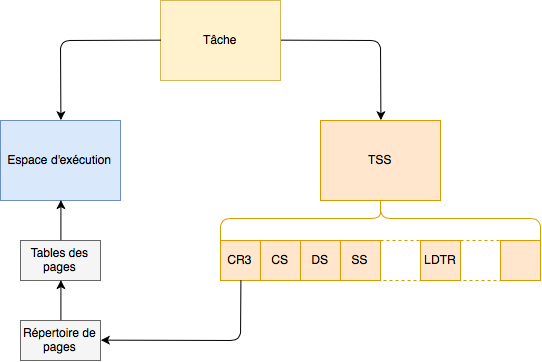
\includegraphics[scale=.7]{images/task_exec_space.png}
  \caption{Structure d'une tâche avec la pagination}
  \label{task_exec_space}
\end{figure}

La structure \acrshort{tss} permet aussi de sauvegarder le contexte de la tâche
dans le cas où une tâche en appelle une autre. Chaque \acrshort{tss} a un descripteur
dans la \acrshort{gdt}. Il y a donc autant de descripteurs de \acrshort{tss} dans
la \acrshort{gdt} que de tâches. Une tâche est alors identifiée par le sélecteur
de segment référençant son \acrshort{tss} dans la \acrshort{gdt} \cite{ref42}. Etant
donné que la pagination est utilisée dans la version finale de notre \acrshort{os},
nous allons nous concentrer sur la gestion des tâches utilisant un répertoire de
pages.

%%%%%%%%%%%%%%%%%%%%%%%%%%%%%%%%%%%%%%%%%%%%%%%%%%%%%%%%%%%%%%%%%%

\subsubsection{Commutation de tâche}
Nous avons vu dans la partie précédente qu'une tâche est divisée en deux parties,
son espace d'exécution et sa structure \acrshort{tss}. Le processeur fourni un
mécanisme permettant de sauvegarder le contexte de la tâche courante et de commuter
vers une nouvelle tâche. La sauvegarde du contexte se fait en utilisant le \acrshort{tss}
lié à la tâche à exécuter et plus particulièrement le sélecteur de ce \acrshort{tss}
dans la \acrshort{gdt}. Ce dernier doit être donné commer argument à l'instruction
\mintinline{text}{ltr}. Cette instruction permet de charger le sélecteur de \acrshort{tss}
dans un registre spécial, le \textit{task register}. Ce registre indique au processeur
quelle est la tâche courante. Lorsqu'une commutation de tâche a lieu, l'état
courant du processeur est automatiquement sauvegardé dans le \acrshort{tss} pointé
par le \textit{task register}. Il est donc nécessaire de créer un \acrshort{tss}
initial avant d'exécuter la première tâche car l'état du processeur doit être
sauvegardé \cite{ref42}. Ci-dessous, la structure \acrshort{tss} en rust.

\begin{minted}[fontsize=\footnotesize,tabsize=4,frame=single]{rust}
pub struct Tss {
    previous_task_link : u16, reserved0    : u16,
    esp0               : u32,
    ss0                : u16, reserved1    : u16,
    esp1               : u32,
    ss1                : u16, reserved2    : u16,
    esp2               : u32,
    ss2                : u16, reserved3    : u16,
    cr3                : u32,
    eip                : u32, eflags       : u32, eax: u32, ecx: u32, edx: u32,
    ebx                : u32, esp          : u32, ebp: u32, esi: u32, edi: u32,
    es                 : u16, reserved4    : u16,
    cs                 : u16, reserved5    : u16,
    ss                 : u16, reserved6    : u16,
    ds                 : u16, reserved7    : u16,
    fs                 : u16, reserved8    : u16,
    gs                 : u16, reserved9    : u16,
    ldt_selector       : u16, reserved10   : u16,
    reserved11         : u16,
    iomap_base_addr    : u16
}
\end{minted}

Dans le \acrshort{tss} initial, seuls les champs \mintinline{rust}{esp0},
\mintinline{rust}{ss0} et \mintinline{rust}{cr3} sont utilisés. Les champs
\mintinline{rust}{esp0} et \mintinline{rust}{ss0} sont utilisés pour stocker
la pile pour le niveau de privilèges 0 et \mintinline{rust}{cr3} doit pointer
sur le répertoire de pages du \textit{kernel}. Ce \acrshort{tss} est ensuite chargé
dans le \textit{task register} avec l'instruction \mintinline{text}{ltr}. Le
\textit{kernel} peut maintenant exécuter une tâche utilisateur. L'architecture
\acrshort{IA-32} offre de nombreux mécanismes pour commuter vers une nouvelle
tâche. La méthode utilisée est un appel explicite à la tâche avec l'instruction
\mintinline{text}{call far}. Cette instruction prend comme argument le sélecteur
du \acrshort{tss} de la tâche à exécuter (comme l'instruction \mintinline{text}{ltr}).
L'initialisation du \acrshort{tss} d'une tâche est légèrement plus complexe que
celle du \acrshort{tss} initial. Les sélecteurs de segment doivent pointer sur les
bons segments dans la \acrshort{gdt}. De plus, le pointeur d'exécution doit
pointer là où commence le code du programme utilisateur et les champs \mintinline{rust}{ss},
\mintinline{rust}{esp} et \mintinline{rust}{ebp} sont utilisés pour stocker la pile
pour le niveau de privilèges 3. L'adresse du début du programme utilisateur dépend
de la manière dont le répertoire de pages de la tâche a été initialisé. Dans notre
cas, le programme utilisateur commence toujours à l'adresse 0x0. Un programme
utilisateur contenu par exemple dans le disque dur peut ainsi être exécuté en
\textit{ring} 3. Ce programme ne pourrait par contre pas faire grand chose car
il n'aurait le droit d'accéder ni aux périphériques, ni à la mémoire. Les appels
systèmes permettent de résoudre ce problème.

%%%%%%%%%%%%%%%%%%%%%%%%%%%%%%%%%%%%%%%%%%%%%%%%%%%%%%%%%%%%%%%%%%
%%%%%%%%%%%%%%%%%%%%%%%%%%%%%%%%%%%%%%%%%%%%%%%%%%%%%%%%%%%%%%%%%%

\subsection{Appels systèmes}
Les appels systèmes sont des fonctions exposés aux applications utilisateur par
le \textit{kernel}. Lors d'un appel système, un changement de privilèges a lieu
car du code du \textit{kernel} est appelé. Il est important d'avoir des appels
systèmes dans un \textit{kernel} appelant des applications utilisateurs car
un programme utilisateur ne pourrait que modifier des variables et appeler des
fonctions s'il ne pouvait pas appeler du code au niveau du \textit{kernel}. Prenons
par exemple un simple affichage texte. Le programme utilisateur étant isolé du reste
de la mémoire, il ne peut pas accéder à la \acrshort{vram} et par conséquent ne
peut rien afficher à l'écran. Les appels systèmes se présentent donc comme une
\acrshort{api} de l'\acrshort{os}. Le mécanisme permettant à du code exécuté en
mode utilisateur d'appeler du code en mode \textit{kernel}
est réalisé grâce à une interruption logicielle choisie et configurée par le \textit{kernel}.
Cette interruption est configurée afin d'être exécutable en \textit{ring} 3.
Dans le cas de notre \textit{kernel}, l'interruption utilisée est la première libre
après les interruptions matérielles. C'est l'interruption 48. Sa configuration se
fait avec le code rust ci-dessous.

\begin{minted}[fontsize=\footnotesize,tabsize=4,frame=single]{rust}
IDT[48] = IdtEntry::new(GDT_KERNEL_CODE_SELECTOR as u16,
                        _syscall_handler as *const () as u32,
                        TYPE_TRAP_GATE, DPL_USER);
\end{minted}

La structure des entrées de l'\acrshort{idt} est décrite dans la figure \ref{idt_entry}.
Dans ce code, le constructeur d'une entrée prend comme argument le sélecteur de
segment pour accéder à l'\acrshort{isr} (ici le sélecteur de segment de code du
\textit{kernel}), le pointeur vers l'\acrshort{isr} en question, le type d'entrée
(ici c'est une \textit{trap gate}) et enfin le niveau de privilèges pour appeler
cette interruption. Ainsi, cette interruption peut être appelée avec l'instruction
\mintinline{text}{INT 48}. A noter qu'une seule interruption logicielle gère tous
les appels systèmes. Ceci est possible car un numéro d'appel système est passé en
argument à la routine d'interruption qui s'occupe d'appeler la bonne fonction.
En général, d'autres paramètres doivent être passés à l'appel système dépendamment
de l'action faite par ce dernier. Par exemple un chaîne de caractères à afficher
à l'écran. Tous ces paramètres sont envoyés à la routine d'interruption dans les
registres du processeur (\mintinline{text}{eax}, \mintinline{text}{ebx}, \mintinline{text}{ecx},
\mintinline{text}{edx} et \mintinline{text}{esi}).

\begin{figure}[!h]
  \centering
  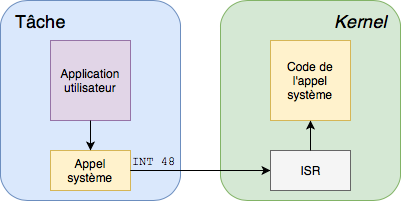
\includegraphics[scale=.75]{images/syscall.png}
  \caption{Fonctionnement des appels systèmes}
  \label{syscall}
\end{figure}

Avec la pagination active, il est important de copier les tables des pages et les
pages du \textit{kernel} dans le répertoire de pages de la tâche. C'est pour cette
raison que nous avons déplacé le \textit{kernel} dans le dernier gigaoctet de
\acrshort{ram} (chapitre \ref{activate_paging}). De cette façon, les trois premiers
gigaoctets de \acrshort{ram} peuvent être utilisés par une application utilisateur
et le reste par le \textit{kernel}.

%%%%%%%%%%%%%%%%%%%%%%%%%%%%%%%%%%%%%%%%%%%%%%%%%%%%%%%%%%%%%%%%%%
%%%%%%%%%%%%%%%%%%%%%%%%%%%%%%%%%%%%%%%%%%%%%%%%%%%%%%%%%%%%%%%%%%

\subsection{Allocation dynamique en mode utilisateur}
